\documentclass{beamer}

\usepackage[utf8]{inputenc}
\usepackage{lmodern} 
\usepackage[utf8]{inputenc}
\usepackage{lmodern} 
\usepackage{listings}
\usepackage{xcolor} 
\usepackage{graphicx}
\definecolor{myblue}{RGB}{48, 63, 159}
\setbeamercolor{palette primary}{bg=myblue, fg=white}
\setbeamercolor{structure}{fg=myblue}
\setbeamercolor{frametitle}{bg=myblue, fg=white}
\setbeamercolor{title}{bg=myblue, fg=white}
\setbeamercolor{footlinecolor}{bg=myblue, fg=white}


\defbeamertemplate*{title page}{mytemplate}{
	\vfill
	\begin{center}
		
		\begin{beamercolorbox}[wd=0.8\paperwidth, center, rounded=true, shadow=true]{title}
			\usebeamerfont{title}\inserttitle\par
		\end{beamercolorbox}
		\vspace{2cm} 
		
		\usebeamerfont{author}\insertauthor
		\vspace{1cm} 
		\usebeamerfont{date}\insertdate
	\end{center}
	\vfill
}


\defbeamertemplate*{frametitle}{mytemplate}{
	\begin{beamercolorbox}[wd=\paperwidth, ht=2.5ex, dp=1.5ex, left]{frametitle}
		\hspace{1em}\usebeamerfont{frametitle}\insertframetitle
	\end{beamercolorbox}
}


\setbeamertemplate{footline}{
	\begin{beamercolorbox}[wd=\paperwidth, ht=2.25ex, dp=1ex]{footlinecolor}
		\hspace{1em}\usebeamerfont{author in footline}\insertshortauthor
		\hfill
		\usebeamerfont{title in footline}\insertshorttitle
		\hfill
		\usebeamerfont{date in footline}\insertdate \hspace{1em} \insertframenumber/\inserttotalframenumber \hspace{0.5em}
	\end{beamercolorbox}
}


\setbeamerfont{author in footline}{size=\tiny}
\setbeamerfont{title in footline}{size=\tiny}
\setbeamerfont{date in footline}{size=\tiny}

\newcommand{\myvec}[1]{\ensuremath{\begin{pmatrix}#1\end{pmatrix}}}
\providecommand{\brak}[1]{\ensuremath{\left(#1\right)}}


\title{8.2.20}
\author{Shriyansh Chawda-EE25BTECH11052}




\begin{document}
\setbeamertemplate{footline}{} 
\frame{\titlepage}
	
\begin{frame}{Question} 
Find the equation of the conic, that satisfies the given
conditions:\\
Vertex (0,0) passing through (2,3) and axis is along X axis.
\end{frame}
	
\begin{frame}{Solution}
The general conic is 
\begin{align}
	g(\vec{x}) = \vec{x}^\top \vec{V}\vec{x} + 2\vec{u}^\top \vec{x} + f = 0
\end{align}
\text{For axis along the $x$-axis, } 
\begin{align}
	\vec{V} = \myvec{A & 0 \\ 0 & C}, \quad 
	\vec{u} = \myvec{D \\ 0}
\end{align}
\text{Since the vertex is at the origin, } 
\begin{align}
	\nabla g(\vec{0}) = 2\vec{u} = \vec{0} 
	\implies \vec{u} = \myvec{0 \\ 0}
\end{align}
If $ \det(\vec{V}) = AC \neq 0,$ then the conic has a center at the origin, which corresponds to an ellipse or hyperbola.\\
But the problem specifies a single vertex at the origin, not a center, so this case is invalid.
\end{frame}



\begin{frame}{Solution}
\begin{align}
	\therefore \det(\vec{V}) = 0 \quad \implies \quad \text{The conic is a parabola.}
\end{align}
\begin{align}
	g(\vec{x}) &= \vec{x}^\top \vec{V}\vec{x} + 2\vec{u}^\top \vec{x} + f = 0 
\end{align}
For a parabola with axis along the $x$-axis, vertex at origin,  
focus $\vec{F} = \myvec{p \\ 0}$ and directrix $\vec{n}^\top \vec{x} = c$,  
we have $\vec{n} = \myvec{1 \\ 0}, \; c = -p$.

\begin{align}
	\vec{V} &= \|\vec{n}\|^2 \vec{I} - \vec{n}\vec{n}^\top 
	= \myvec{1 & 0 \\ 0 & 1} - \myvec{1 \\ 0}\myvec{1 & 0} 
	= \myvec{0 & 0 \\ 0 & 1}
\end{align}
\begin{align}
	\vec{u} &= c\vec{n} - \vec{F} 
	= (-p)\myvec{1 \\ 0} - \myvec{p \\ 0} 
	= \myvec{-2p \\ 0}
\end{align}	
\end{frame}

\begin{frame}{Solution}
 \begin{align}
 	f &= \|\vec{F}\|^2 - c^2 = p^2 - (-p)^2 = 0
 \end{align}
 Thus, the parabola equation becomes:
 \begin{align}
 	&\vec{x}^\top \myvec{0 & 0 \\ 0 & 1}\vec{x} 
 	+ 2\myvec{-2p & 0}\vec{x} + 0 = 0\\
 	&y^2 - 4px = 0
 \end{align}
 Since $(2,3)$ lies on the parabola:
 \begin{align}
 	3^2 - 4p(2) &= 0 \\
 	9 - 8p &= 0 \\
 	p &= \frac{9}{8}
 \end{align}
 Therefore,
\end{frame}

\begin{frame}{Solution}
Therefore,the equation of the required parabola is
\begin{align}
	y^2 = \frac{9}{2}x
\end{align}
\end{frame}


\begin{frame}{Plot}
\begin{figure}[H]
	\centering
	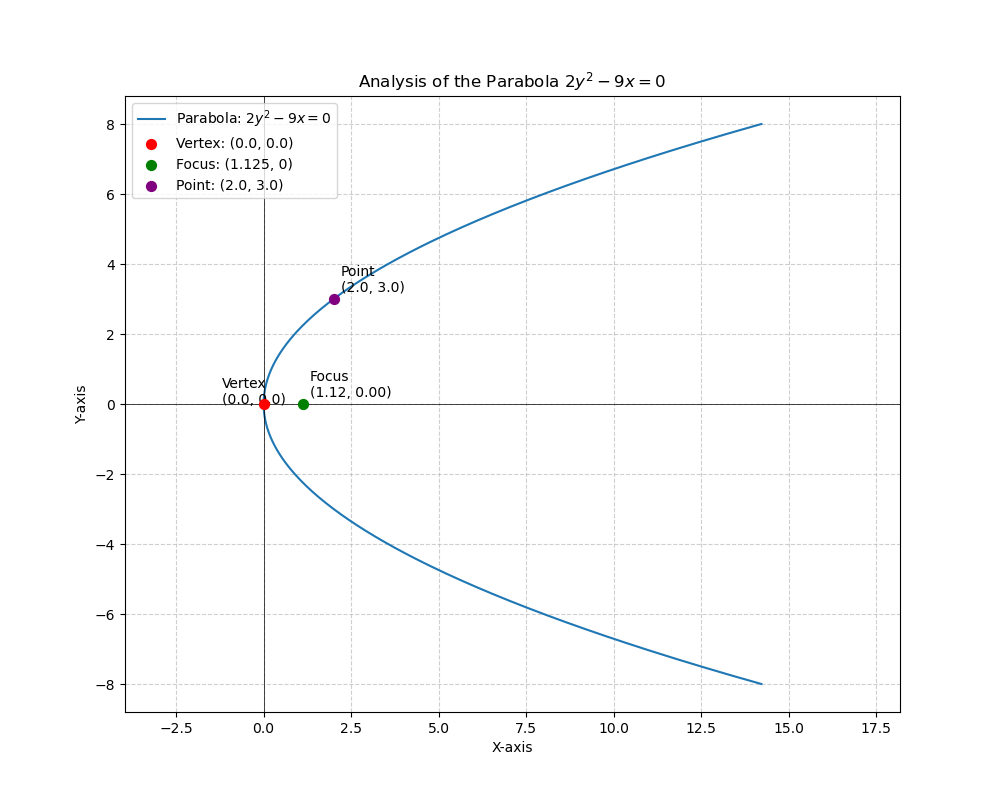
\includegraphics[width=1\linewidth]{figs/parabola}
\end{figure}


\end{frame}
\end{document}